% %        ************************************************
% %        **	LaTeX preamble to be used with all 
% %	**	statsTeachR labs/handouts.
% %
% %	Author: Eric A. Cohen
% %	Last modified: 22 August 2013
% %	************************************************
% 
\documentclass[table]{beamer}\usepackage[]{graphicx}\usepackage[]{color}
%% maxwidth is the original width if it is less than linewidth
%% otherwise use linewidth (to make sure the graphics do not exceed the margin)
\makeatletter
\def\maxwidth{ %
  \ifdim\Gin@nat@width>\linewidth
    \linewidth
  \else
    \Gin@nat@width
  \fi
}
\makeatother

\definecolor{fgcolor}{rgb}{0.345, 0.345, 0.345}
\newcommand{\hlnum}[1]{\textcolor[rgb]{0.686,0.059,0.569}{#1}}%
\newcommand{\hlstr}[1]{\textcolor[rgb]{0.192,0.494,0.8}{#1}}%
\newcommand{\hlcom}[1]{\textcolor[rgb]{0.678,0.584,0.686}{\textit{#1}}}%
\newcommand{\hlopt}[1]{\textcolor[rgb]{0,0,0}{#1}}%
\newcommand{\hlstd}[1]{\textcolor[rgb]{0.345,0.345,0.345}{#1}}%
\newcommand{\hlkwa}[1]{\textcolor[rgb]{0.161,0.373,0.58}{\textbf{#1}}}%
\newcommand{\hlkwb}[1]{\textcolor[rgb]{0.69,0.353,0.396}{#1}}%
\newcommand{\hlkwc}[1]{\textcolor[rgb]{0.333,0.667,0.333}{#1}}%
\newcommand{\hlkwd}[1]{\textcolor[rgb]{0.737,0.353,0.396}{\textbf{#1}}}%

\usepackage{framed}
\makeatletter
\newenvironment{kframe}{%
 \def\at@end@of@kframe{}%
 \ifinner\ifhmode%
  \def\at@end@of@kframe{\end{minipage}}%
  \begin{minipage}{\columnwidth}%
 \fi\fi%
 \def\FrameCommand##1{\hskip\@totalleftmargin \hskip-\fboxsep
 \colorbox{shadecolor}{##1}\hskip-\fboxsep
     % There is no \\@totalrightmargin, so:
     \hskip-\linewidth \hskip-\@totalleftmargin \hskip\columnwidth}%
 \MakeFramed {\advance\hsize-\width
   \@totalleftmargin\z@ \linewidth\hsize
   \@setminipage}}%
 {\par\unskip\endMakeFramed%
 \at@end@of@kframe}
\makeatother

\definecolor{shadecolor}{rgb}{.97, .97, .97}
\definecolor{messagecolor}{rgb}{0, 0, 0}
\definecolor{warningcolor}{rgb}{1, 0, 1}
\definecolor{errorcolor}{rgb}{1, 0, 0}
\newenvironment{knitrout}{}{} % an empty environment to be redefined in TeX

\usepackage{alltt}


%       ************************************************
%       **        LaTeX preamble to be used with all 
%	**        statsTeachR labs/handouts.
%
%	Author: Nicholas G Reich
%	Last modified: 14 January 2014
%	************************************************

% \documentclass[table]{beamer}

%	Set theme (a nice plain one)
\usetheme{Malmoe}

%	Use named colors, set main color of theme
%		to match Web site color:
\definecolor{MainColor}{RGB}{10, 74, 109}
\colorlet{MainColorMedium}{MainColor!50}
\colorlet{MainColorLight}{MainColor!20}
\usecolortheme[named=MainColor]{structure} 

%	For tables
%[dvipsnames] [table]
\usepackage{xcolor}
\usepackage{tabu}	% Even fancier than tabulary
\usepackage{multirow}

%	Just for the degree symbol
\usepackage{textcomp}

%	Get rid of footline (page, author, etc. on each slide)
\setbeamertemplate{footline}{}
%	Get rid of navigation buttons
\setbeamertemplate{navigation symbols}{}

%	Make footnotes not ugly
\usepackage{hanging}
\setbeamertemplate{footnote}{\raggedright\hangpara{1em}{1}\makebox[1em][l]{\insertfootnotemark}\footnotesize\insertfootnotetext\par}

%	Text style for code snippets inline in text:
\newcommand{\codeInline}[1]{\texttt{#1}}

%	Text style for emphasis stronger than \emph:
%		(Note, this doesn't toggle the way \emph does.
%			(Note, this can be done, didn't seem worth the trouble.))
\newcommand{\strong}[1]{{\bfseries{#1}}}


%        ******	Define title page	**********************
\setbeamertemplate{title page}{
	{\color{MainColor}
	% There must be a better way than this -vspace at
	%	 the top and bottom of the page to reduce the 
	%	 bottom margin, but I can't find one that works.
	\vspace{-6em}

% 	% Go to a lot of trouble to get the title in a
% 	%	nice box, since customizing a beamer block
% 	%	does not entirely work here (I don't know why)
	\newlength{\titleBoxWidth}
	\setlength{\titleBoxWidth}{\textwidth}
	\addtolength{\titleBoxWidth}{-2.0em}
	\setlength{\fboxsep}{1.0em}
	\setlength{\fboxrule}{0pt}
	\fcolorbox{MainColor!25}{MainColor!25}{
		\parbox{\titleBoxWidth}{
			\raggedright
			\LARGE\textbf{\inserttitle}
		}	% end parbox
	}	% end fcolorbox

	\vfill
	\small{Author: \insertauthor}
	\vspace{\baselineskip}

	\small{\Course}

	\small{\Instructor}
	\vspace{\baselineskip}

	\small{\emph{This material is part of the \strong{statsTeachR} project}}

	\vspace{0.33\baselineskip}\scriptsize{\emph{\LicenseText}}


		\vspace{-15em}

	}	% end color
	\clearpage
}	% end define title page

%        The following variables are assumed by the standard preamble:
%	Global variable containing module name:
\title{}
%	Global variable containing module shortname:
%		(Currently unused, may be used in future.)
\newcommand{\ModuleShortname}{bigGWASdata}
%	Global variable containing author name:
\author{Nicholas G Reich}
%	Global variable containing text of license terms:
\newcommand{\LicenseText}{Made available under the Creative Commons Attribution-ShareAlike 3.0 Unported License: http://creativecommons.org/licenses/by-sa/3.0/deed.en\textunderscore US }
%	Instructor: optional, can leave blank.
%		Recommended format: {Instructor: Jane Doe}
\newcommand{\Instructor}{}
%	Course: optional, can leave blank.
%		Recommended format: {Course: Biostatistics 101}
\newcommand{\Course}{}


\usepackage{multicol}
\IfFileExists{upquote.sty}{\usepackage{upquote}}{}

\begin{document}





\title{BiP 2014: Module 4}


\author{Andrea S. Foulkes}


\begin{frame}[plain]
        \titlepage
\end{frame}

\begin{frame}{Genome Wide Association Studies (GWAS)}

\emph{The overarching \underline{\bf goal} of genome wide association studies is to identify genes associated with complex traits.}

\bigskip
Three broadly-defined data components:
\begin{enumerate}
\item Genetic information
\item Trait (phenotype) measuring disease progression or status
\item Demographic and clinical covariates 
\end{enumerate}
\begin{figure}[ht]
\fbox{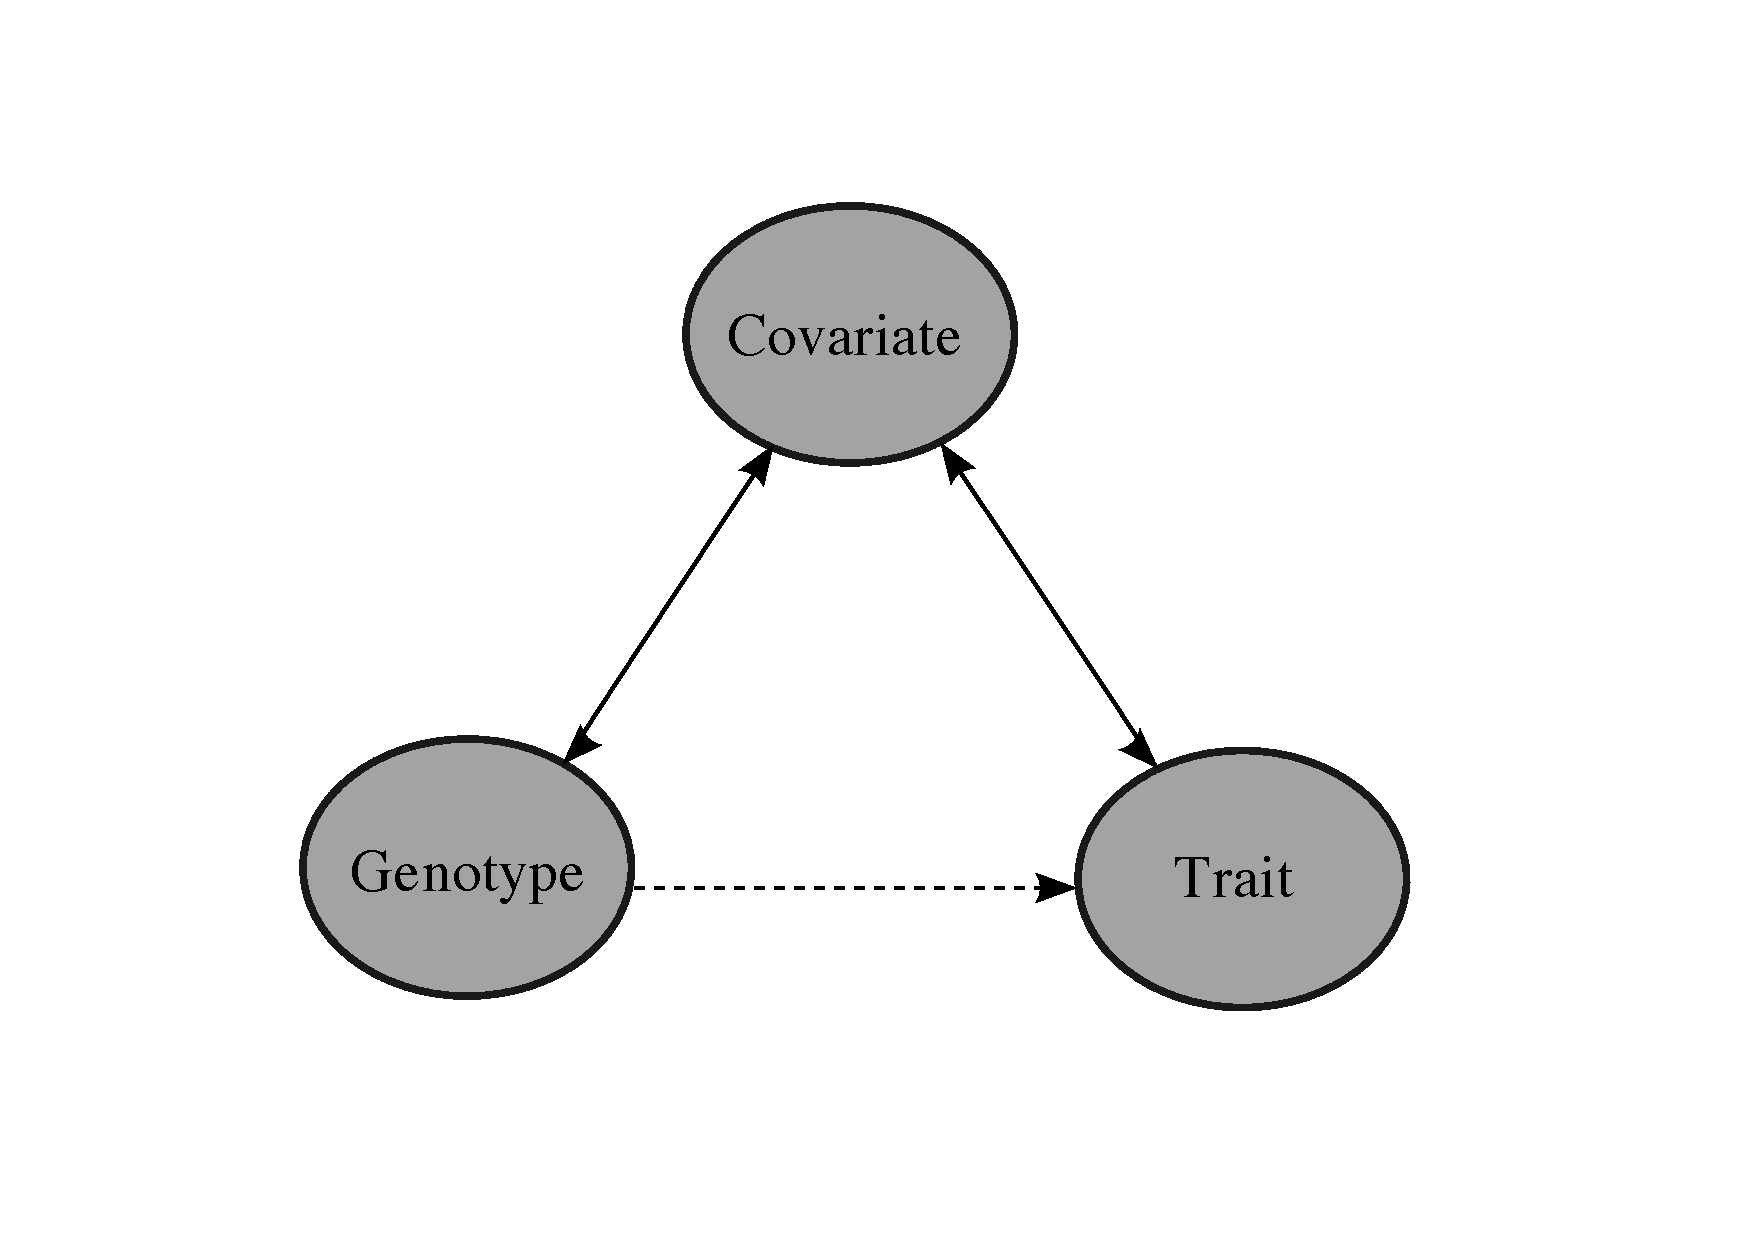
\includegraphics[width=0.5\textwidth]{Pictures/covariate.pdf}}
\end{figure}
\end{frame}

\begin{frame}{Data components and terminology}
Genetic information
\begin{itemize}
\item Humans carry 2 \emph{homologous chromosomes}:
  \begin{itemize}
	\item segments of DNA, one inherited from each parent.
	\item code for same trait, may carry different genetic information.
	\end{itemize}
\item \emph{Nucleotide}:
	\begin{itemize}
	\item DNA base + sugar molecule + phosphate.
	\item used interchangeably with \emph{base}.
	\end{itemize}
\item Gene:
	\begin{itemize}
	\item region of DNA
	\item code for proteins or involved in regulation of production of proteins from other segments of DNA
	\end{itemize}
\end{itemize}
\end{frame}
	
\begin{frame}{Data components and terminology}
\begin{multicols}{2}
\centerline{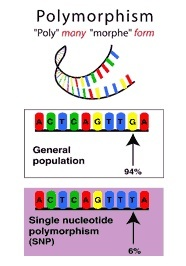
\includegraphics[scale=.6,angle=0]{polymorphism2.jpg}}
\vspace{.25in}
\begin{itemize}
\item SNP ($x$): basic unit of analysis, typically coded 0, 1, 2 for number of variant alleles on 2 chromosomes
\item Trait ($y$): measure of disease progression or disease status.
\end{itemize}
\end{multicols}
\scriptsize
\underline{Definitions}: 
\begin{enumerate}
\item[-] {\bf polymorphism}: genetic variant occurring in greater than $1\%$ of a population
\item[-] {\bf single nucleotide polymorphism (SNP)}: variant at a single site (base pair position) on the genome.
\end{enumerate}

\end{frame}

\begin{frame}
\fbox{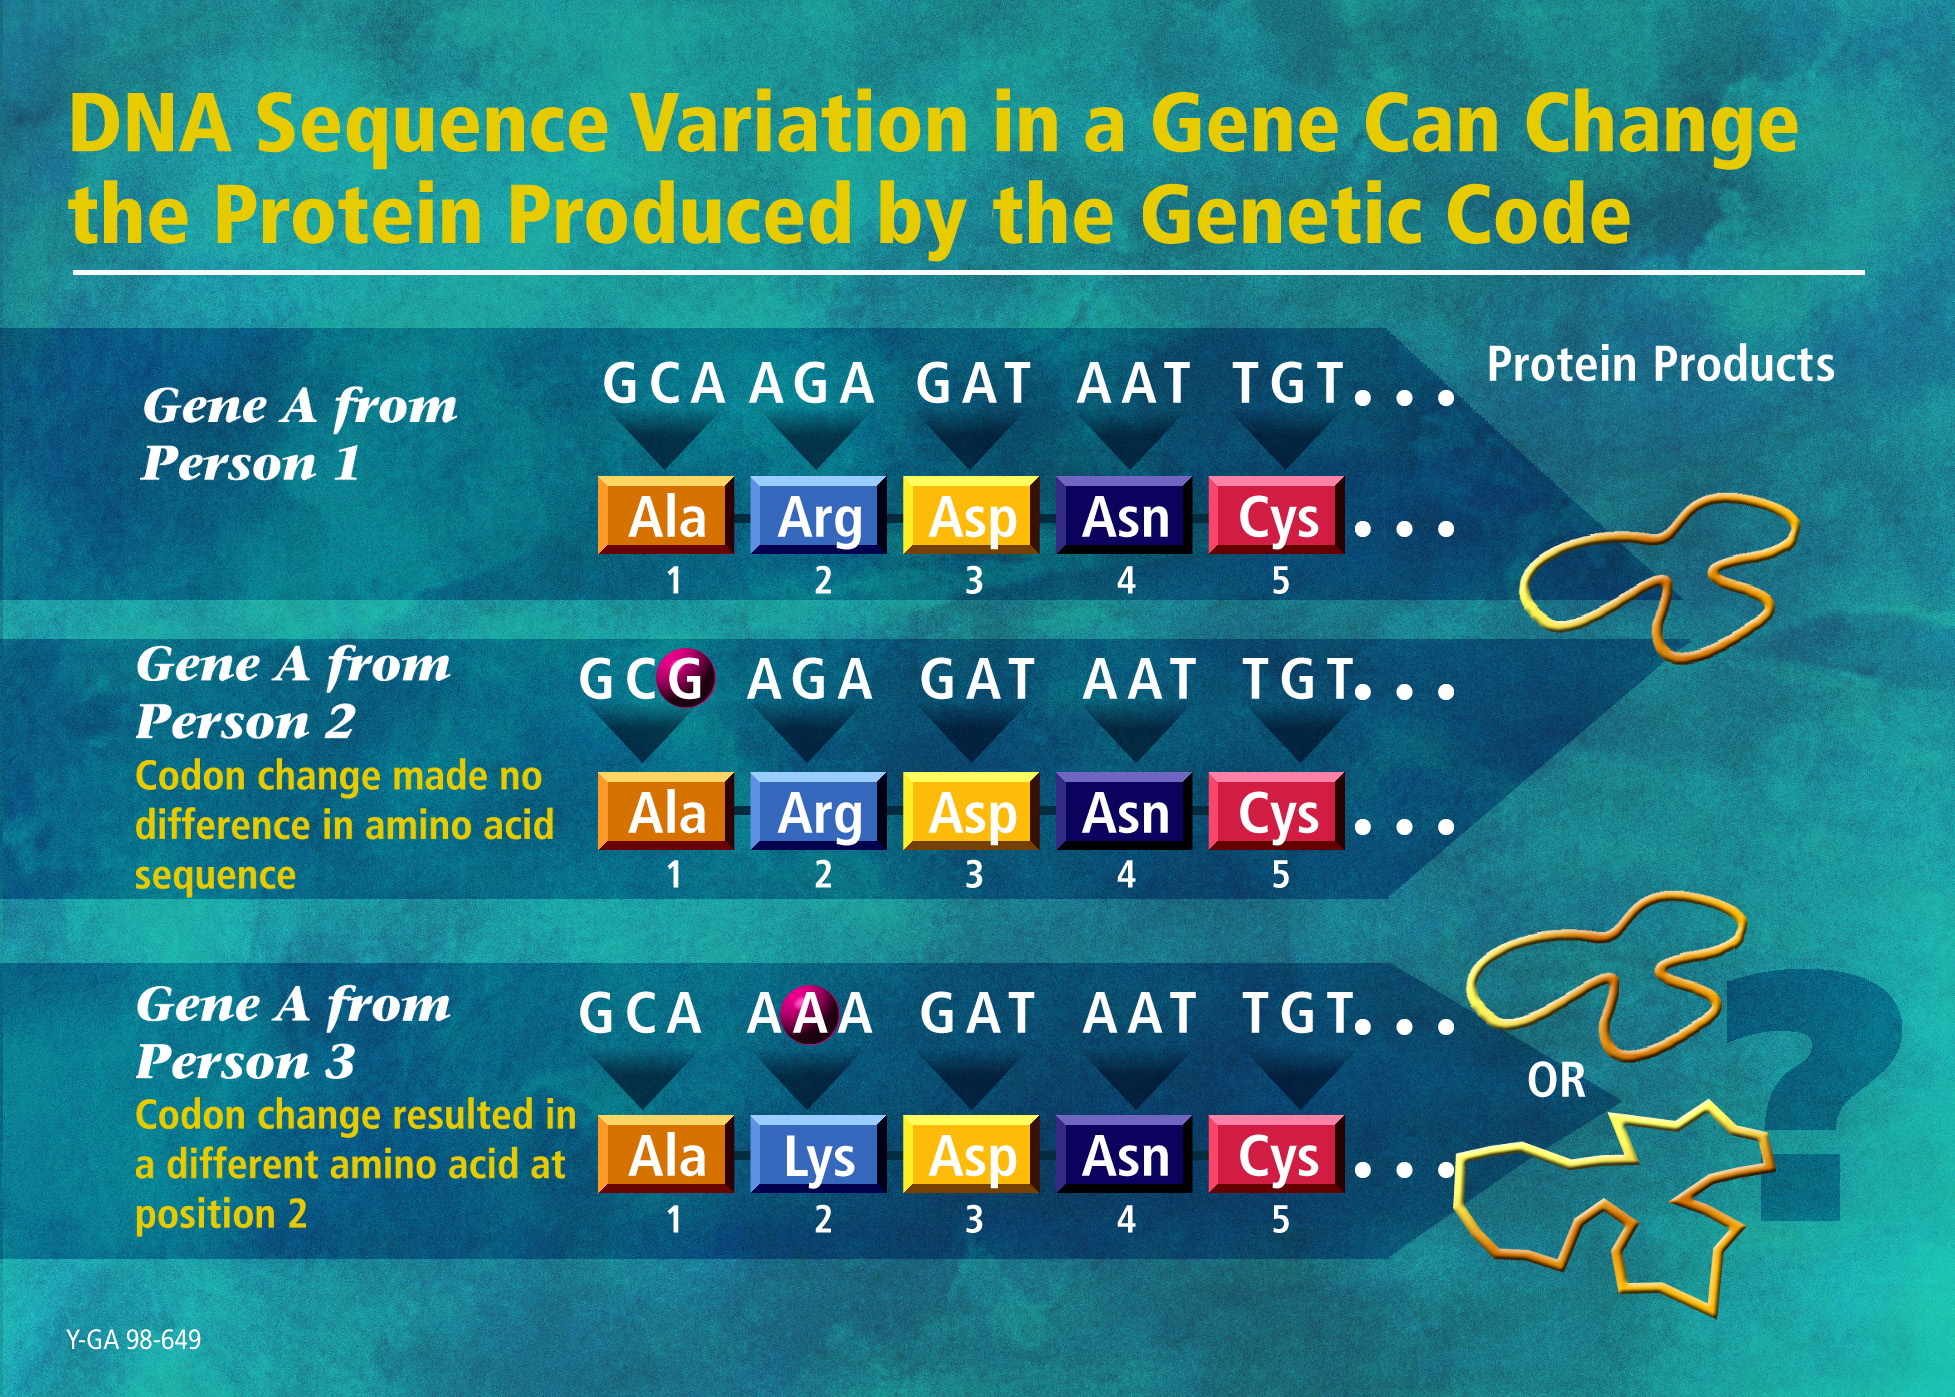
\includegraphics[angle=0,width=.9\textwidth]{Pictures/SNPtoAA.jpg}}
\end{frame}


\begin{frame}{Data components and terminology}
\fbox{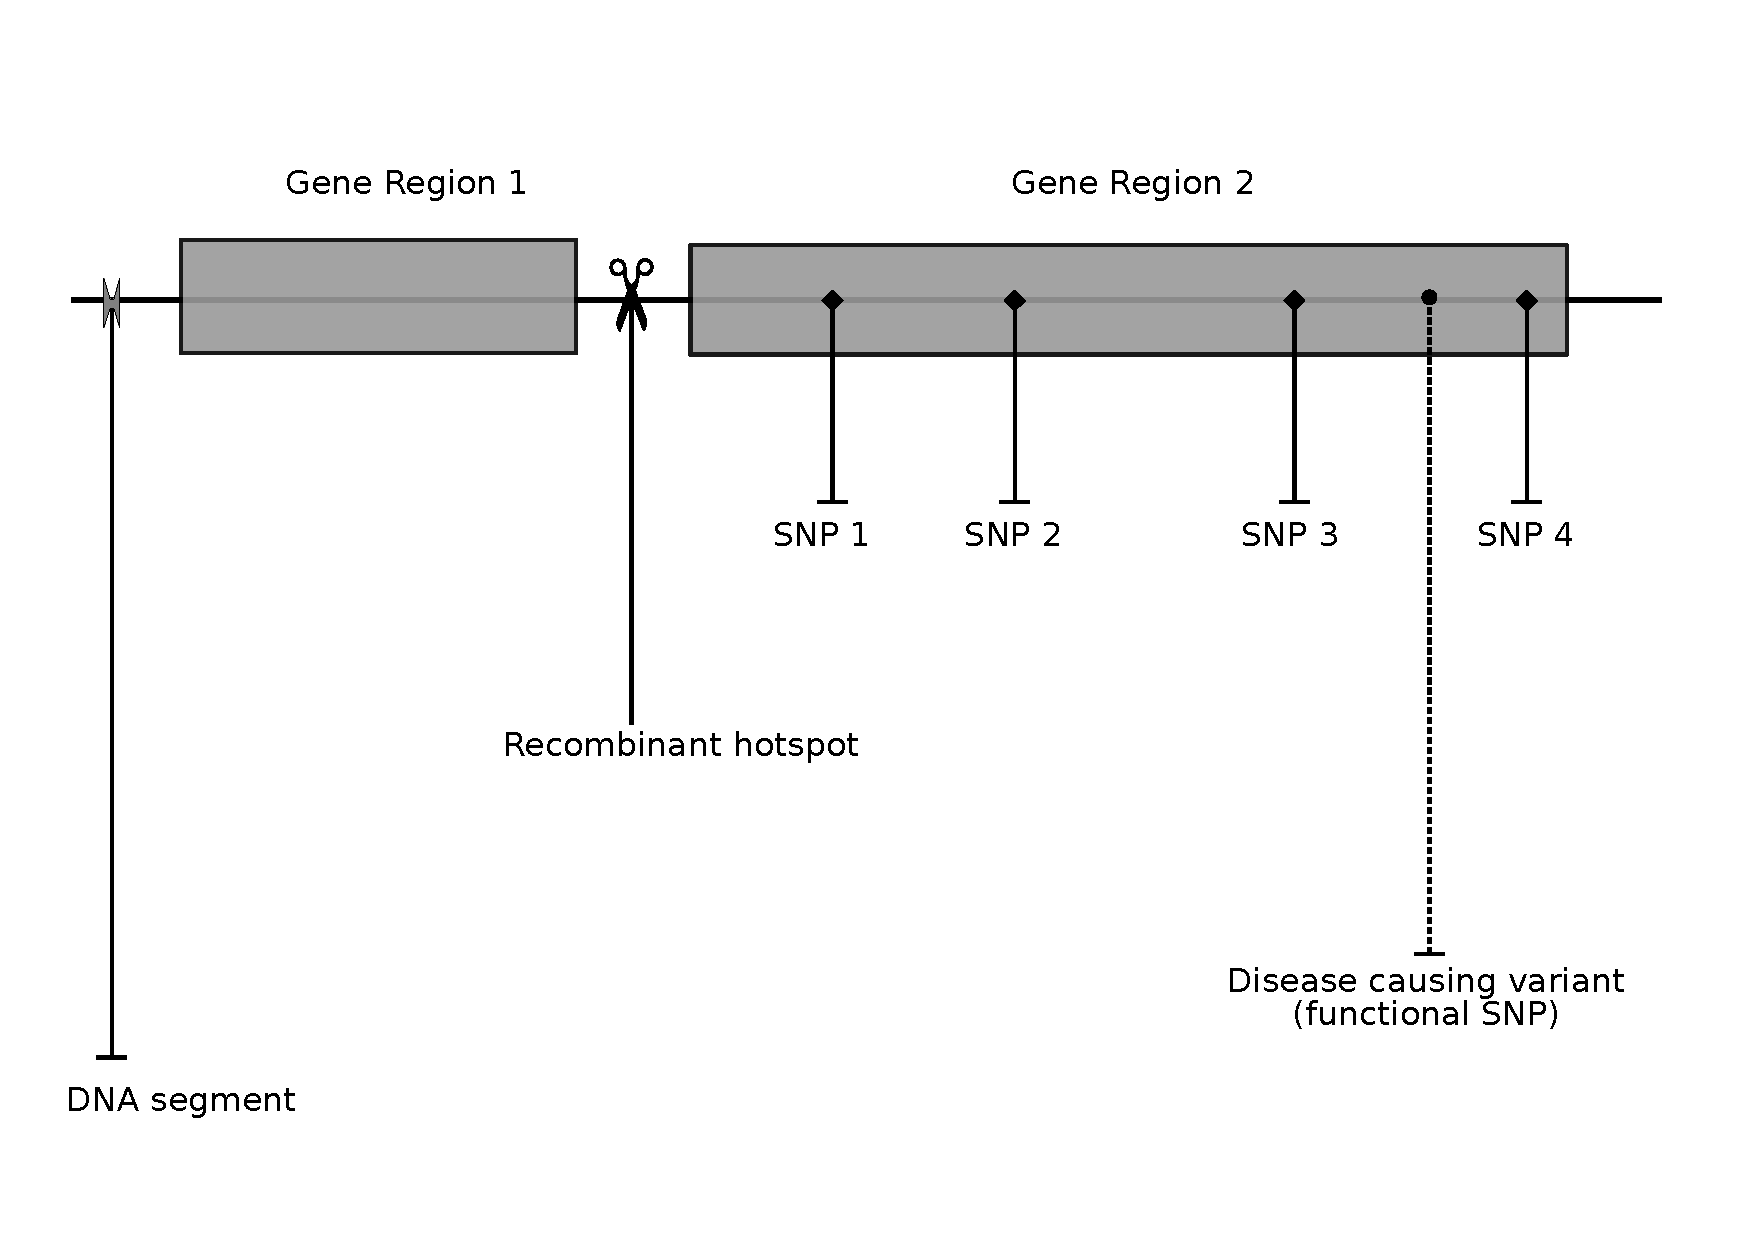
\includegraphics[angle=0,width=1\textwidth]{ldblocks.pdf}}
\end{frame}

\begin{frame}{Data components and terminology}
\fbox{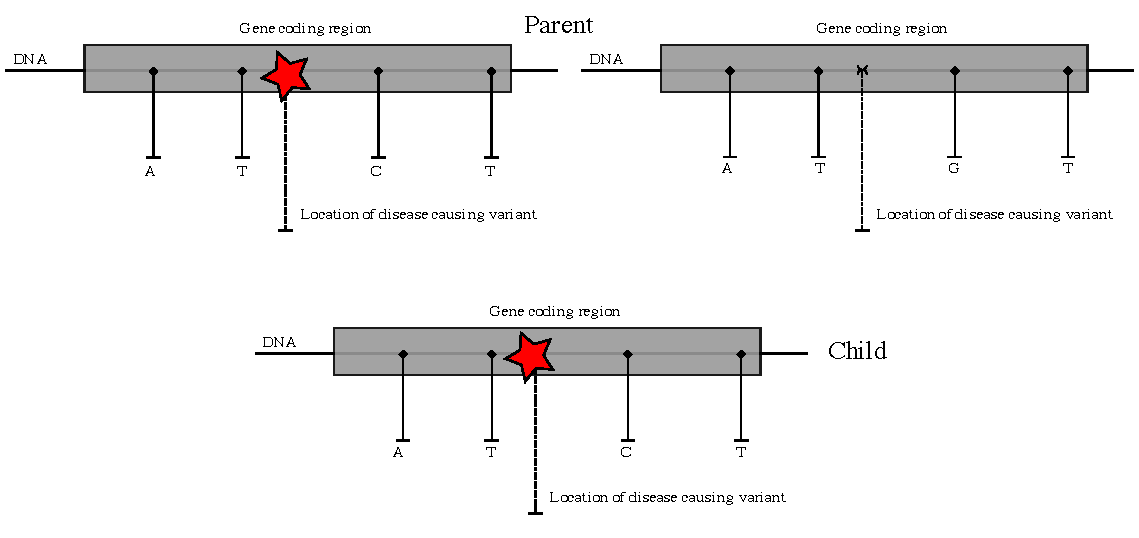
\includegraphics[angle=0,width=1\textwidth]{Pictures/markers_inherit.pdf}}
\end{frame}

\begin{frame}{Data components and terminology}
\fbox{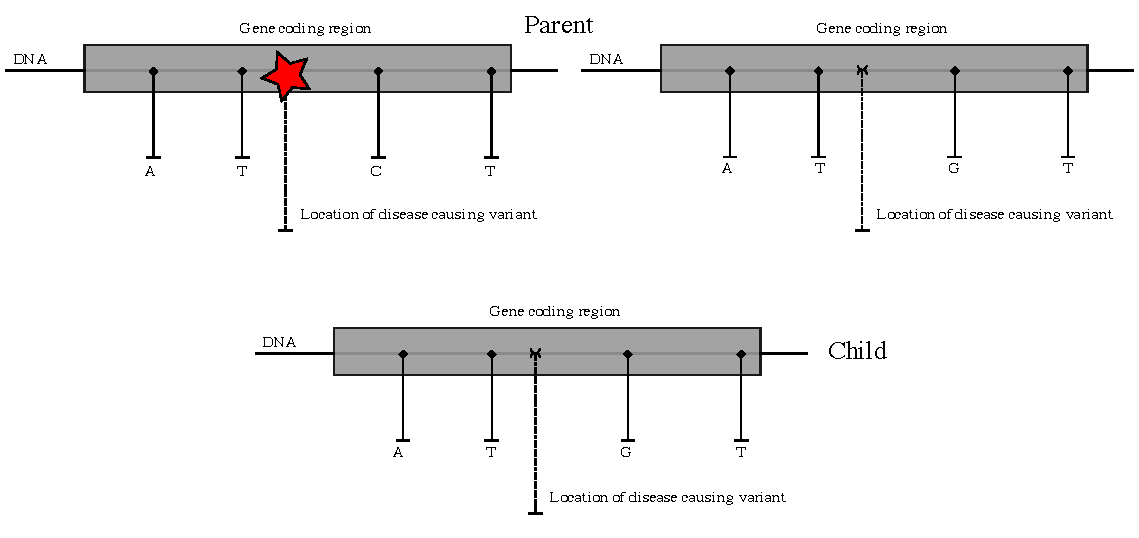
\includegraphics[angle=0,width=1\textwidth]{Pictures/markers_inherit2.pdf}}
\end{frame}

\begin{frame}{Data components and terminology}
Trait
\begin{itemize}
\item clinical outcome or phenotype, measured \emph{in vivo} or \emph{in vitro}.
\item {\bf quantitative}, {\bf binary} (diseased or not diseased), survival (censored), longitudinal/multivariate.
\item e.g. total cholesterol, triglyceride levels, heart attack, CD4+ cell count, viral load, AIDS defining event, time to death, repeated measures of total cholesterol, etc.
\end{itemize}
Covariates
\begin{itemize}
\item environmental, clinical and demographic data.
\item potential predictors, confounders, effect modifiers, effect mediators (causal pathway variables).
\item also referred to as \emph{predictors}, \emph{confounders}, \emph{explanatory variables}, \emph{independent variables}.
\item e.g. age, gender, race/ethnicity, BMI, smoking status, etc.
\end{itemize}
\end{frame}


\begin{frame}{GWAS Analysis}
``Typical" analysis approach:
\begin{itemize}
\item Separate test of association (based on multivariable linear model) for each SNP $\rightarrow$ p-value for each SNP.

\begin{equation*}
Y=X\beta + Z \gamma + \epsilon
\end{equation*}

\begin{equation*}
H_0: \beta=0
\end{equation*}

\item Adjust to control Family Wise Error Rate (FWER) in context of multiple testing: 

\begin{equation*}
FWER=Pr(\text{reject at least one }H_0^k \; | \text{all } H_0^k \text{ are true})
\end{equation*}

\item Typically control at level $\alpha=0.05$ using Bonferonni adjustment $\rightarrow$ P-value statistically significant if less than $0.05/1,000,000=-5 \times 10^{-8}$.
\end{itemize}
\end{frame}

\begin{frame}{CARDIoGRAM summary level data}

{\bf C}oronary {\bf AR}tery {\bf DI}sease {\bf G}enome-wide {\bf R}eplication {\bf A}nd {\bf M}eta-anaylsis (CARDIoGRAM) data:

\begin{itemize}
\item Meta-analysis of 14 GWAS of coronary artery disease (CAD): 22,233 cases and 64,762 controls
\item Replication study in additional $56,682$ individuals
\item Available data (after pre-processing): p-values for $965,220$ SNPs in $19,216$ genes.  
\end{itemize}
\end{frame}

\begin{frame}
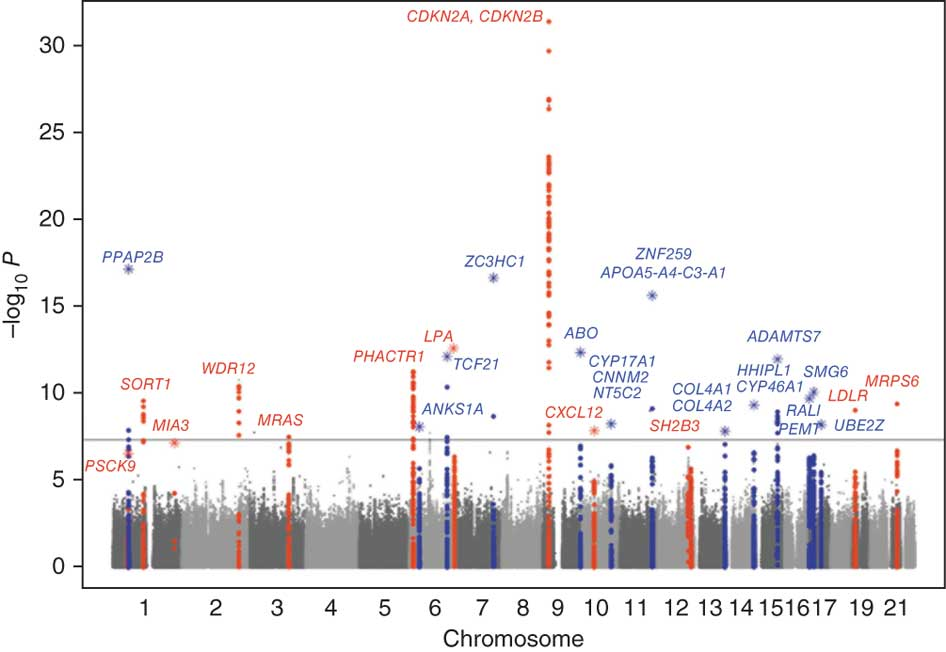
\includegraphics[angle=0,width=1\textwidth]{ng784-F1.jpg}

\scriptsize Schunkert et al. Nature Genetics 43,  333-338 (2011) doi:10.1038/ng.784
    
\end{frame}

\begin{frame}{Lab Assignment}
\begin{enumerate}
\item Conduct a simulation study to identify an appropriate p-value threshold for statistical significance (assuming independence of SNPs):
\begin{itemize}
	\item generate $965,220$ p-values from a uniform distribution
	\item determine value corresponding to the $5$th percentile
	\item repeat $500$ times and record $5$th percentile of this distn.
	\end{itemize}
\item Repeat (1) while accounting for within gene correlation
	\begin{itemize}
	\item assume inverse normally transformed p-values ($p_{ij}$) arise from a random effects model (i indicates gene and j indicates SNP):
	
	\begin{equation*}
	y_{ij}= b_i +\epsilon_{ij}
	\end{equation*}
	
	$p_{ij}=\Phi^{-1}(y_{ij})$, $b_i \sim N(0,0.4)$, $\epsilon_{ij} \sim N(0,1)$ and $b_i \perp \epsilon_{ij}$.
	 
	\end{itemize}
\item Repeat (2) where the random gene level effects arise from a $N(0,\sigma_b^2)$ and $\sigma_b^2$ ranges from 0.2 to 1.2 in increments of 0.2. 
\end{enumerate} 
\end{frame}



\end{document}
